\documentclass[nofootbib,floatfix,11pt]{article}
\usepackage[square]{natbib}
\usepackage[paperwidth=8.5in,paperheight=11in,centering,margin=1in]{geometry}
\usepackage{paralist}
\usepackage{parskip}

\setlength{\parindent}{3ex}

\usepackage[compact,medium]{titlesec}
\titlespacing{\part}{0pt}{*0}{2ex}
\titlespacing{\section}{0pt}{2pt}{1ex}
\titlespacing{\subsection}{0pt}{2pt}{1ex}
\titlespacing{\subsubsection}{0pt}{*0}{1ex}
\titleformat*{\section}{\large \bf}
\titleformat*{\subsection}{\bf}
\titleformat*{\subsubsection}{\itshape}

% suck up extra white space
\setlength{\parskip}{3pt}
\setlength{\parsep}{0pt}
\setlength{\headsep}{0pt}
\setlength{\topskip}{0pt}
\setlength{\topmargin}{0pt}
\setlength{\topsep}{0pt}
\setlength{\partopsep}{0pt}

\renewcommand{\thefootnote}{\alph{footnote}}
\setlength{\belowcaptionskip}{-10pt}

\usepackage{amsmath}
\usepackage{amsbsy}

\usepackage{epsfig}
\usepackage{color}
\usepackage{subfigure}
\usepackage{graphicx}

%commented out the line below to get rid of citations that run into margins
%\usepackage{multicol}

%\usepackage{etoolbox}

%\renewcommand{\baselinestretch}{0.971}

\usepackage{hyperref}


\title{Statistical Explorations of Data in the {ACMS} {Program} at the {University} of {Washington}}
\author{PI: Marina \meila, Co-PIs: Andrew Connolly, \v{Z}eljko Ivezi\'{c}, Jacob Vanderplas}

%%%%%%%%%%%%%%%%%%%%%%%%%%%%%%%%%%%%%%%%%%%%%%%%%%%%%%%%%%%%%%%%%%%%%%%
\font\math = cmmi12
\newcommand\x         {\hbox{$\times$}}
\hyphenation{para-met-ri-zed Qua-sars cross-vali-da-tion}
%%%%%%%%%%%%%%%%%%%%%%%%%%%%%%%%%%%%%%%%%%%%%%%%%%%%%%%%%%%%%%%%%%%%%%%%%%%%%%%%
%% Commands added by MMP 
\newenvironment{itemize*}{
\begin{itemize}
\setlength{\parskip}{0em}
\setlength{\topskip}{0em}
}
{\end{itemize}}

\newenvironment{enumerate*}{
\begin{enumerate}
\setlength{\parskip}{0em}
\setlength{\topskip}{0em}
}
{\end{enumerate}}

\newcommand{\comment}[1]{}
\newcommand{\mmp}[1]{\textcolor{red}{#1}}

\newcommand{\meila}{Meil\u{a}}
\newcommand{\cdse}{CDS\&E}

\newcommand{\astroml}{{\tt AstroML}}
\newcommand{\astrocl}{{\sc Astr 497}}
\newcommand{\statcl}{{\sc Stat 391}}

\newcommand{\bit}{\begin{itemize}}
\newcommand{\eit}{\end{itemize}}
\newcommand{\bits}{\begin{itemize*}}
\newcommand{\eits}{\end{itemize*}}
\newcommand{\benum}{\begin{enumerate}}
\newcommand{\eenum}{\end{enumerate}}
\newcommand{\benums}{\begin{enumerate*}}
\newcommand{\eenums}{\end{enumerate*}}


%%%%%%%%%%%%%%%%%%%%%%%%%%%%%%%%%%%%%%%%%%%%%%%%%%%%%%%%%%%%%%%%%%%%%%%%%%%%



\begin{document}

% we don't need title - it's done automatically by Fastlane
%\maketitle

\section{ INTRODUCTION}

This three-year project is an enthusiastic response to the EXTREEMS-QED (Expeditions in Training, Research, 
and Education for Mathematics and Statistics Through Quantitative Explorations of Data) solicitation for proposals
that aim to train the next generation of statistics and mathematics undergraduate students for confronting new
challenges in computational and data-enabled science and engineering (\cdse).  The proposed work addresses and 
includes all the main required project components: Education and Training, Research, and Faculty Professional 
Development. The proposed program will provide opportunities for undergraduate research and hands-on experiences 
centered on \cdse\ and will result in significant changes to the undergraduate mathematics and statistics curriculum 
at the University of Washington. We have secured broad institutional support and buy-in from two major departments 
(Statistics and Astronomy), and the proposed work includes a workshop centered on professional development activities
for faculty from other institutions wishing to emulate the proposed program. 

\vskip 0.1in Our main goals and deliverables are: 
\bits
\item {\bf Education and Training} (Section \ref{sec:education}).

Transform the ACMS (Applied and Computational Math Sciences) Program Statistics track
\begin{itemize}
  \item two new courses
  \item new curriculum 
  \item undergraduate \cdse~ Research Seminar
  \end{itemize}
\item {\bf Research and mentoring for research} (Section \ref{sec:research})
\begin{itemize}
  \item facilitate entrance of Statistics students into computationally intensive data analysis research
  \item mentoring of undergraduate students by PI, Co-PIs, and graduate students
  \item mentoring of Statistics and Astronomy graduate students by PI and Co-PIs
  \end{itemize}
\item {\bf Dissemination and Outreach} (Section \ref{sec:outreach})

 \bits
  \item software and datasets infrastructure for teaching computational statistics and machine learning 
  \item workshop for UW faculty % in the use of the infrastructure and our experience with it
  \item workshop with outside participation. 
 \eits
\eits  

In the remainder of this proposal, we describe each component in
detail, how they fit within the ACMS program and the overall ``Big
Data'' efforts within the University of Washington, and the budget and
execution schedule for the proposed program.


  % the same
   
\section{Education and Training}
\label{sec:education}
\subsection{\bf About the ACMS program}

The ACMS {\em (Applied and Computational Mathematical Sciences)} was
introduced in 1998 as a joint undergraduate program between the
departments of Applied Mathematics, Computer Science and Engineering
(CSE), Mathematics, and Statistics, among others.

The ACMS program is structured into a {\em core} set of courses,
totaling 43 credits, and a set of options, or {\em tracks}. The tracks
are either associated with a particular application domain (Biological
and Life Sciences, Mathematical Economics, Social and Behavioral
Sciences, Engineering and Physical Sciences) or with a particular area
of specialization in the mathematical sciences ({\em Discrete Math and
  Algorithms, Operations Research, Scientific Computing and Numerical
  Analysis, and \underline{Statistics}}).

It is the Statistics track of ACMS that we are aiming to
tranform. Currently, this track contains, in addition to the core
courses, the following:
\\
{\bf Option Core (37 credits)}
\bits
    \item {\sc PHYS 121-2-3} (replaceable by other courses in application areas)
    \item {\sc STAT 302} Statistical Software and Its Applications (R course, irregularly offered, 2 credits)
    \item {\sc STAT 340} Probability and Mathematical Statistics
    \item {\sc STAT 341-2} to Probability and Statistical Inference I,II
    \item {\sc STAT 421} Applied Statistics and Experiment Design
    \item {\sc STAT 423} Applied Regression and Analysis of Variance
\eits
{\bf Option Electives (10 credits)}
\bits
    \item {\sc MATH/STAT 396} Probability III
    \item {\sc MATH/STAT 491-2} Stochastic Processes
    \item {\sc STAT 403}  Resampling Inference
    \item {\sc STAT 427}  Analysis of Categorical Data
    \item {\sc STAT/BIOST 529} Sample Survey Techniques
    \item {\sc CSE 373} Data Structures
    \item {\sc MATH 300} Mathematical Reasoning
    \item {\sc MATH 327}  Real Analysis I
    \item {\sc MATH 407--8--9} Linear, Nonlinear,\& Discrete Optimization
    \item {\sc STAT 428} Multivariate Analysis for the Social Sciences
    \item {\sc GEOG 426} Quantitative Methods in Geography
    \item {\sc QMETH 528} Survey Sampling Applications
    \item {\sc STAT 498} Special topics
\eits
The program web page recommends that ``[this track] is ideally suited as a {\em second major} for students with a primary focus in the [\ldots] sciences''.
De facto, the track curriculum differs little, most notably by the
presence of the computer programming class {\sc CSE 142}, from the
``standard'' Statistics major.

{\bf Enrollment} The ACMS major is competitive, with the number of
majors capped at about 200.  During the recent academic years,
graduation numbers have passed 100 students per year; the current
enrollment is at 147\footnote{Complete breakdown of ACMS graduation
  numbers from 1998 on are in the Supplementary material.}.  Of these,
the Statistics track accounts for 4 students currently enrolled (none
as double majors), and for 2 to 6 students graduated in each of the
last 5 years. In the same time, enrollment in the Statistics major is
at an all times high, with \mmp{fill} of which XX women.

\subsection{Transforming the Statistics  ACMS track}
We will transform the ACMS Statistics track into a virtually new
major, a ``computationally minded Statistics major focused on Big Data''. 
In other words, we will not aim to produce scientists who also know statistics (which
can be well served by Statistics minor and other tracks of ACMS) but
full-fledged statisticians who can function autonomously in the modern
cyberworld.

There are several motivating factors:
\bit
\item Interest in statistics is at an all times high, as witnessed by
  our enrollment numbers. We expect that the ACMS Statistics track
  will reach similar enrollment numbers. Note that at the current
  enrollment in the other tracks, the total ACMS enrollment will be
  near the 200 level.

\item The role of
  the statistician as data analyst has become both more central, and
  more demanding. As more data analysis and more decisions based on it
  are being shifted from humans to computers, statistics is called
  upon to design and validate the procedures used to take these
  decisions. Thus, the statician's importance in a much wider range of
  human activities, be they science or business. But the
  statistician's responsibility is commensurately growing, as (s)he needs
  to master the skills required by cyber-enabled science and data
  analysis.
\item These skills are not limited to using computers and
  programming. The nature of statistical analyses itself is
  affected \mmp{get some citations} as it has been long
  recognized. Computationally heavy statistical methods need to be
  designed. Very large samples will support models of a complexity
  that could not be considered in real-life scenarios a decade or two
  ago. It is now not possible to perform model selection by explicitly
  comparing all possible models (i.e. there can be an exponential
  number of models to compare) and regularization methods are often
  called into play, as are approximate computational
  techniques. Leveraging unlabeled data for prediction is now an
  almost universal necessity. Devising new methods to evaluate complex
  models in an environment that is not stationary, nor controlled are
  some of the challenges of modern data analysis.
\item The proposal fits in and leverages other \cdse\ efforts and successes at UW in creating a strong collaborative environment for (the e-science Institute, the IGERT for graduate education in Big Data and the related PhD tracks recently created in CSE and Statistics). The time is ripe to involve undergraduates, and specifically statistics and mathematics majors in this change.
\item This proposal is in the spirit of the ACMS original mission,
  bringing this part up to speed with the demands of the coming decade.
\eit

{\bf Work Plan}

For planning purposes, we divide the proposed project into three stages which
roughly map to yearly schedule. 

{\bf Stage 1:} Design and introduce two new courses \statcl, \astrocl,
as {\em electives} in the track.  Start the Undergraduate \cdse~
Research Seminar. This seminar will differ from the existing ``ACMS''
Undergraduate Math Science Seminar ({\sc Math 498}), in that the
speakers will be undergraduates themselves or their mentors, and the
seminar topics will be their projects (see Section
\ref{sec:ugrad-seminar} for more details).

{\bf Stage 2:} Redesign the track: move \statcl, Stochastic Processes {\sc STAT 481, 482} into the core. As the track will no longer be regarded as a second major for science students, we will make room by removing the {\sc PHYS 121-2-3} courses (15 credits) from it.  Reorganizing the electives into two groups: math/stat electives (group I) and computing and science electives (group II). Further reorganization of the core and electives in consultation with Statistics faculty and the other ACMS participating departments and Schools. For example, we will consider adding one or both of {\sc AMATH 482, 483} ``Data analysis'', ``High performance scientific computing''.

Organization of a workshop for UW faculty to share our experiences and teaching infrastructure.

{\bf Stage 3:} Incorporate feedback from evaluators and all participants. Continue developing the courses' software and data infrastructure. 

In addition to this plan, although we are at the moment not explicitly
proposing this, we will investigate if the two new courses could be
made accessible to Mathematics majors as well. Mathematics Professor
William Stein, creator and leader of the {\tt Sage} project, teaches a
successful Python programming course in Mathematics, which could serve
to build a pathway towards one or both of the two new courses, if a
way to satisfy the Statistics prerequisites is also found.


{\bf Why this particular approach?} Currently, computer education is
assured primarily through two core courses, {\sc CSE 142, 143}
\cite{cse142}. These set the foundations in the understanding of
computer programming, but they are of a general nature, and are mainly
focused towards preparing future programmers  (these courses are the
same courses that the approximately 500 CSE majors take). Thus, there
is no room for data analysis applications in these courses.  There is
also a programming in R course ({\sc STAT 302}, 2 credits) but it is 
offered quite irregularly.

However, for reasons we will expound later (Section \ref{sec:Python}), we
consider that Python is the more appropriate computer language for our
goals. Thus, we will both introduce Python and will use it to teach
statistical methodology.  As Python will be taught as a second
programming language, and as it is similar enough to Java (taught in
CSE 142), we expect the students to assimilate it quickly under our
guidance (there are also numerous publicly available tutorials).
In Spring 2013, a pilot course was taught (by H. Koepke,
Statistics) that introduced Python and taught statistical modeling
using the language, to an audience of around 40 CSE undergraduates
(the vast majority of wich did {\em not} know Python). The students'
feedback was very encouraging, and one of the reasons we are confident
in our approach.

The need for a dedicated scientific computing course was long
recognized, hence the Scientific Computing track and courses developed
by AMATH {\sc 481} (project based, in Matlab) {\sc 482}, and {\sc 483}. 
Our proposed courses are not replicating, but adding a new dimension to
the existing AMATH courses. The latter focus on the ``signal
processing'' aspects of data analysis (e.g filtering, {\sc AMATH
  482}) and on the ``hardware, software, and programming for
large-scale scientific computing'' ({\sc AMATH 483}), while our
courses focus on the statistical modeling and statistical decision
making aspects.
 
\comment{

next steps: other math majors?, new certificates, programs

MMP -find out about minors

will also help students in hard/soft sciences 


\section{University involvement}

UW context: e-sci, igert, phd tracks in stat, cse,..., 
stat context: increased interest in stats/data sci Statistics is recognized (by students themselves) at the forefront of the data science revolution. Phd track, MS track.

Astro involvement

How does UW support this plan:



}%end comment

\subsection{Description of the courses}
\label{sec:course-descr}

\bits
\item \statcl 
``Computational Statistical Modeling and Machine Learning'' (4 credits)
\item \astrocl ``Data Intensive Astronomy'' (3 credits)
\eits
These courses' aims are explicitly to (1) to give students a hands-on experience, through programming, and performing real data analyses on a computer, with the computational aspects of 
statistical modeling in general, and (2) to introduce them to the  machine learning methodology in particular, with specific attention to the issues of big data.

The material covered will be partly overlapping with other courses
(e.g. regression, probability models for discrete data) and partly new
(e.g. classification, clustering). However, the treatment of the
material will stress on the interaction of computational and
statistical aspects in modeling and prediction with scientific and
engineering data. In this sense, the overlap has not been avoided on purpose
so that the students can gain a new, computational, perspective on areas
already studied from a more theoretical point of view. 

{\bf Prerequisites} (for either course): an introductory programming
course (not necessarily in Python), e.g. CSE 142 or equivalent
programming experience; an introductory statistics course; mathematics
multivariate calculus. The two courses can be taken in a sequence
\statcl--\astrocl, or separately. These course can be accessible to
other juniors and seniors with a strong quantitative background.

\bit
\item  \underline{\statcl~ Draft Syllabus}\\
  - a review of the concept of likelihood and Max Likelihood estimation (cases in which MLE has no closed form, gradient ascent/Newton estimation of MLE)\\
  - a review of basic probability models with focus on ML estimation of these models, supported heavily by simulation (e.g demonstrating gaussianity of MLE for certain models, and non-gaussianity for other models, including Zipf's law type distributions)\\
  - models for statistical prediction, with focus on classification\\
  - review and computational aspects of other statistical topics like
  density estimation, clustering, model selection and validation
  (including regularization and  nonparametric modeling)\\
  - intro to programming in Python, and to Python libraries supporting scientific computing\\
  - examples of real applications from engineering and sciences (image
  analysis, information retrieval, etc.)

\item[]{\bf Learning goals for \statcl} Ability to perform computationally intensive, automated, robust and efficient data analysis. Ability to combine existing tools and libraries with programming in a general purpose language (Python). 
Working knowledge of the most important/main machine learning tools and methods, as well as their probabilistic interpretation. Understanding of the practical implications of theoretical results like independence, overfitting, consistency of an estimator. 

{\bf Textbooks} Unfortunately, there is no single textbook one can
assign for this course. We will rely partly on \meila's previously
developed course notes for {\it ``Probability and Statistics for
  Computer Science''}, a computationally minded introductory course,
partly on new course notes to be developed by \meila\ specifically for
this more advanced course, and partly on the textbook of \astrocl, 
which will provide among others the Python exercises. We are also
considering a new machine learning book written for undergraduate
students \cite{x}. 

\comment{
\item{Motivation for \astrocl} \mmp{shorter,more to the point of grant}
Astronomy and astrophysics are witnessing dramatic increases in data volume 
as detectors, telescopes, and computers become ever more powerful. During the 
last decade, sky surveys across the electromagnetic spectrum have collected 
hundreds of terabytes of astronomical data for hundreds of millions of sources. 
Over the next decade, the data volume will enter the petabyte domain, and provide 
accurate measurements for billions of sources. Astronomy and physics students 
are not traditionally trained to handle such voluminous and complex data sets. 
Furthermore, standard analysis methods employed in astronomy often lag far 
behind rapid progress in statistics and computer science. The main
goal of this course is to contribute to efficient training of next
generations of students to 
handle the fast growing data sets, not only in astronomy, but in other quantitative 
sciences as well. 

This course will be aimed at physical and data-centric math,
statistics, science and engineering students
who have an understanding of the science drivers for analyzing large data sets but 
may not be aware of appropriate statistical techniques for doing so. The course work 
will provide to students a connection between scientific data analysis problems and 
modern statistical methods. We will limit theoretical discussions to the minimum 
required to understand the algorithms and will build the courses upon an 
example-driven compendium of modern statistical and data mining methods, 
together with carefully chosen examples based on real modern data sets, and of 
current astronomical applications that will illustrate each method introduced in the 
book. Discussion of the advanced material will be supported by appropriate (publicly 
available) Python code and data which will enable students to perform exercises, 
evaluate the techniques, and adapt them to their own fields of interest. We chose to 
use Python, a powerful and flexible programming language that is quickly becoming 
a standard in data-intensive sciences (and elsewhere). 

The target audience for our course includes undergraduate students
with scientific or engineering background, but it is likely that
graduate students would benefit from it too. Familiarity with calculus
and other basic mathematical techniques will be assumed, but no
extensive prior knowledge in statistics will be required.
}

\item \underline{\astrocl~ Draft Syllabus}\\

Computational Challenges in data-intensive astronomy and astrophysics: \\
- data types and data management systems \\
- types of computational problems and strategies for speeding them up \\
- data visualization challenges \\
- selection effects and truncated/censored data in astronomical context \\

Exploratory techniques and searching for structure \\
- non-parametric density estimation \\
- cluster finding methods (focus on non-parametrics and large data) \\

Dimensionality reduction\\
- review of principal component analysis in a large data context \\
- non-negative matrix factorization  \\
- independent component analysis and projection pursuit \\

Regression and model fitting for large data \\
- applications using real data from large sky surveys \\

Basics of time series analysis \\
- applications using real data from large sky surveys \\

Adoption and development of cross-disciplinary tools (e.g. numerical 
algorithms, visualization methods, data-human interaction) in the context
of big data, astronomical or otherwise (see Section \ref{sec:Python}).
\eit

{\bf Learning goals for \astrocl} \\
- familiarity with drivers for and accomplishments of modern astronomical surveys\\
- ability to perform computationally intense/automated and efficient data analysis\\
- ability to combine existing tools and libraries with programming in a general purpose language (Python)\\
- working knowledge of the most important/main machine learning tools and \\
   methods, as well as their probabilistic interpretation \\
- help to develop a diverse STEM workforce \\
 


{\bf Textbook} {\it ``Statistics, Data Mining, and Machine Learning in
  Astronomy: A Practical Python Guide for the Analysis of Survey
  Data''} (Princeton Series in Modern Observational Astronomy),  
coauthored by the Co-PIs on this proposal.

{\bf Format and student experience} 
The courses will consist of lectures, homework assignments, 1--2
miniprojects, and a final exam. The TA will hold quiz sections; about
half of these will be in a (virtual) computer lab environment. 

{\bf The Computer Lab recitations} will offer support for learning
Python, as well as specific data analysis tools (see Section \ref{sec:Python}).
The students will practice programming in pairs (a.k.a extreme
programming), using debuggers, profilers, writing modifiable code, etc.

Another experience in the computer lab will be actual data analysis
and visualization using the tools, the skills related to data
visualisation, experimental data recording and reporting, etc.

{\bf Homework assignments} There will be 4-5 homework
assignments. They will contain concept problems, algorithmic problems,
programming assignments, and data analysis assignments.

A note on the overlap between \statcl~ and \astrocl: Where the two
courses have overlapping topics, \astrocl~ will consider the big data case
explicitly, while \statcl~ will be considering the connections between
statistical theory and computation. \statcl~ will support more basic
Python, while \astrocl~ will support Python libraries for big data.


\subsection{Python Packages} 
\label{sec:Python}

\begin{figure*}[!t]
\vskip -1.8in
\includegraphics[width=1.02\hsize,clip]{astroML.eps}
\vskip -2.0in
\caption{We will leverage all the modern Python tools available in {\it astroML} and
other packages, including a large number of practical data-intensive exercises developed to
support textbook that will be used with the proposed \astrocl~ course.} 
\label{Fig:astroML}
\end{figure*}


We will leverage all the publicly available modern Python tools. In particular, seminar work will be 
built around the {\it astroML} package (available from http://www.astroml.org) that was developed 
by Co-PIs to support the textbook to be used with the proposed \astrocl course. {\it astroML} is a Python module 
for machine learning and data mining built on {\it numpy}, {\it scipy}, {\it scikit-learn}, and {\it matplotlib}, 
and distributed under the 3-clause BSD license. It contains a growing library of statistical and machine 
learning routines for analyzing astronomical data in Python, loaders for several open astronomical datasets, 
and a large suite of examples of analyzing and visualizing astronomical datasets (there are close to two 
hundred examples of machine learning and visualization in the code library that supports the textbook 
alone). In addition to  {\it astroML} package, we will expose students to several other popular and widely
used toolkits (e.g. PyMC for Markov chain Monte Carlo methods, and HealPy for spherical coordinates 
and spherical harmonic transformations). 

As an example of methods and exercises available in  {\it astroML}, we single out methods 
for reducing data dimensionality. Many astronomical analyses must address the question of the 
complexity as well as size of the data set. Dimensionality reduction methods address the
complexity issue  by finding the directions within a multivariate data set that contain most 
of the information. Classical approaches for identifying the principal dimensions include
principal component analysis (PCA), independent component analysis (ICA), and non-negative 
matrix factorization (NMF). These methods are implemented in   {\it astroML}, with a user-friendly 
interface and adequate documentation (see Figure~\ref{Fig:astroML}). Furthermore, {\it astroML} also 
includes easy-to-use code to automatically access and download spectra collected by the Sloan Digital 
Sky Survey (currently a ``gold standard'' for modern astronomical surveys and big data sets; see sdss.org). 
Therefore, an undergraduate student will not only be exposed to modern statistical methods
and a cutting-edge astronomical data set, but will be empowered to actually apply these methods 
to a real complex and massive data set.  The result of this exercise is shown in Figure~\ref{Fig:astroML2}. 
With such a positive experience, it is very likely that students would not have difficulties applying 
the same methods and tools later to scientifically unrelated but mathematically similar problems.  


\begin{figure*}[!t]
\vskip -1.8in
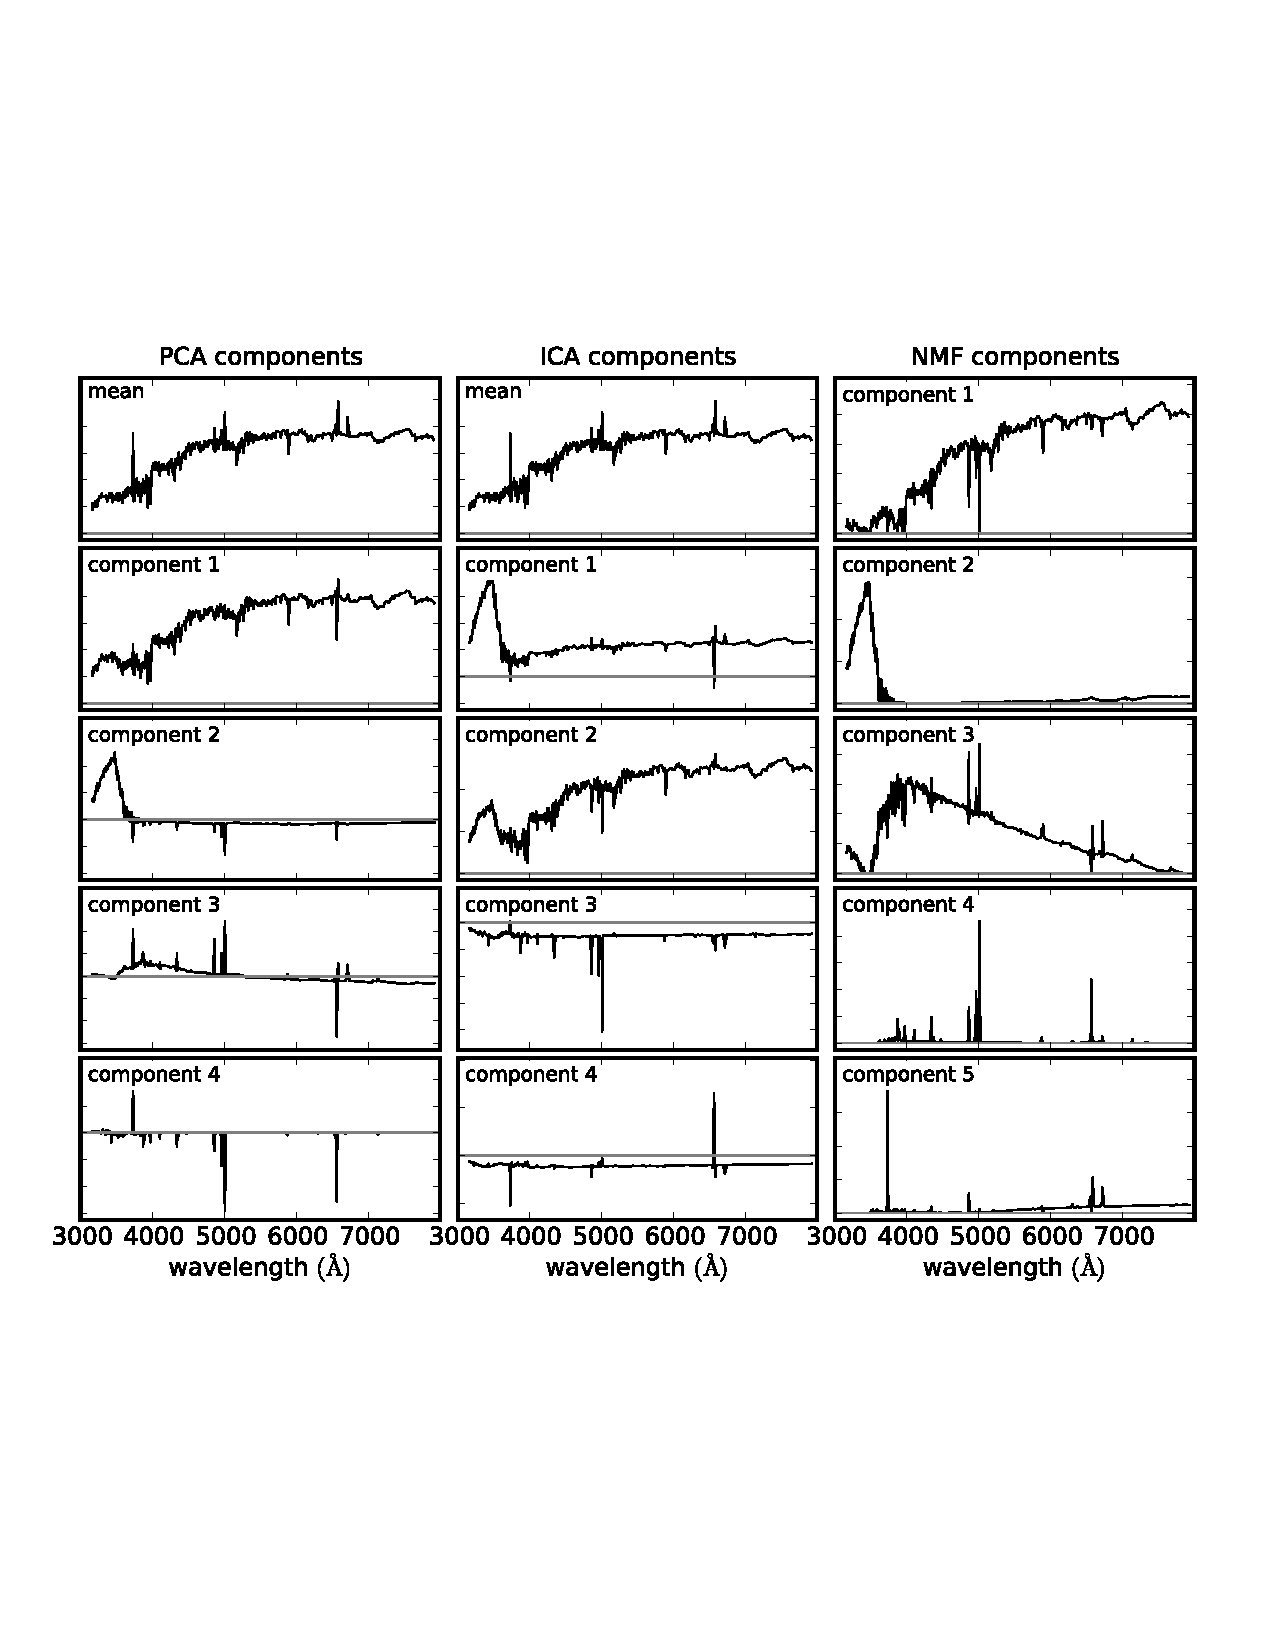
\includegraphics[width=1.02\hsize,clip]{astroML2.pdf}
\vskip -2.0in
\caption{An example of sophisticated tools available in {\it astroML} and exercises that will be
used in practical seminar work. The figure shows a comparison of the decomposition of SDSS 
spectra using PCA (left panel), ICA (middle panel) and NMF (right panel). The rank of the component
increases from top to bottom. For the ICA and PCA the first component is the mean spectrum (NMF 
does not require mean subtraction). All of these techniques isolate a common set of spectral features 
(identifying features associated with the continuum and line emission). The ordering of the spectral 
components is technique dependent. The SDSS spectroscopic database contains over a million
such spectra.} 
\label{Fig:astroML2}
\end{figure*}


\subsection{What we are building on?}
\label{sec:precursors}

\meila~ has extensive previous experience teaching computational
statistics courses at all levels. She developed the
course ``Probability and Statistics for Computer Science'' an
introductory course aimed at computer science majors, complete with exercises and demos in Matlab, revised the Statistical Computing graduate course sequence, later developed the Statistical Learning graduate sequence and led, with prof. Emily Fox, 
the effort to introduce the Machine Learning/Big Data PhD track in the Statistics department. 

\comment{
 under the same
course number \statcl. This has been taught for 11 years at full
enrollment (50 students). From it, what can be transferred to teaching
computing and algorithms to young statisticians? The power of hands on
experience with data, through programs one understands, the
combination of algorithmics and statistics that comes into play for
large, high-dimensional data sets \mmp{clean this up}}

%ZI, AC, JVdP


\meila\ and Connoly co-taught an extremely well received course at CMU
in 1999-2000, ``Computational Statistics of Multi-Dimensional
Scientific Databases'', which reunited students from Statistics,
Computer Science and Astronomy, as well as faculty from these
departments.

The Statistics department runs a {\em Virtual computer lab} that will
be used by \statcl~ students in their quiz sessions and assignments.
%The clusters {\tt newton1,2}, consisting of 8, respectively 2 high memory nodes, 
The high-memory computer clusters, 
accquired from a UW Student Technology Grant, will serve as
basis for the graduate student research. 
% \mmp{shall i buy more nodes??}

The \astroml~ book and web site (see Section \ref{sec:Python}) will provide the starting 
point for the new courses' software and data infrastructure.


\comment{
(Recently, starting 2011, CSE created their own introduction to
probability and statistics, {\sc CSE 312}. Thus it is clear that
\statcl~ can not serve its original purpose and audience.)
\mmp{keep this?}
Therefore, in Spring 2013, the PI \meila with Hoyt Koepke, revised the
course, having in mind that \bit
\item the audience was now literate in statistics and probability
\item the course could now be opened to a larger audience 
\eit
I opted to replace the introductory material with more advanced topics, and for these I chose a set of basic machine learning topics. I also introduced more substantial data analysis assignments. These changes were implemented by Hoyt Kopke, who taught the class. The course web page is at {\tt }. The student feedback to this pilot experiment was very encouraging. \mmp{specifics: how many students, what depts, they liked being made to learn Python, loved the projects too, level was demanding}
}


\comment{OTHER USEFUL INFO
\item These courses fit very well with the original goal and mission of the  ACMS program. 
\item Crosscultural diversity: these classes can also serve science and CSE majors as well as other quantitatively able students across the UW.

{\bf Links}\\
 \statcl Spring 2013 web site {\tt http://www.stat.washington.edu/courses/stat391/spring13/}\\
\astroml~ textbook web site {\tt http://www.amazon.com/Data-Mining-Machine-Learning-Astronomy/dp/0691151695}\\



AMATH 481 Scientific Computing (5)
Project-oriented computational approach to solving problems arising in the physical/engineering sciences, finance/economics, medical, social, and biological sciences. Problems requiring use of advanced MATLAB routines and toolboxes. Covers graphical techniques for data presentation and communication of scientific results. Prerequisite: AMATH 301; either AMATH 351 or MATH 307; either AMATH 352 or MATH 308. Offered: A. 

AMATH 482
Exploratory and objective data analysis methods applied to the physical, engineering, and biological sciences. Brief review of statistical methods and their computational implementation for studying time series analysis, spectral analysis, filtering methods, principal component analysis, orthogonal mode decomposition, and image processing and compression. Prerequisite: AMATH 301; either AMATH 352 or MATH 308. Offered: W.

AMATH 483 High-Performance Scientific Computing (5)
Introduction to hardware, software, and programming for large-scale scientific computing. Overview of multicore, cluster, and supercomputer architectures; procedure and object oriented languages; parallel computing paradigms and languages; graphics and visualization of large data sets; validation and verification; and scientific software development. Prerequisite: either CSE 142 or AMATH 301. Offered: Sp. 

}     % planMarina.tex, plan.tex
\section{RESEARCH PROGRAM}
\label{sec:research}

The research plan under this grant will have as its primary goal to
introduce and prepare students to perform research in computationally
intense statistical modeling and in the statistical analysis of large
scientific data. The students targeted will be Statistics and ACMS
Statistics track undergraduates, as well as Statistics and Astronomy
graduate students. 

We will specifically foster working in teams including graduate and
undergraduate students. The students will be mentored by the four
PI's. They will be working on real research projects, some of which
are listed below. 
\bits
\item {\em Non-linear dimension reduction in large scientific data} is a long-time research interest of \meila, with methodological results in \cite{x}. Currently, these methods have been used largely for data visualisation in Astronomy as well as in other scientific fields; however, we believe they could be useful beyond visualisation, in discovering low dimensional meaningful parametrizations of high-dimensional data. The students will work on implementing scalable Python versions of the algorithms, suitable for large data sets, and, co-advised by the PI's will apply them to the study of scientific data.
\item {\em Non-parametric clustering and density estimation.} We will
  focus here on methods that cluster by finding high-density regions
  in very large data. This method is particularly suited to finding
  non-spherical (or non-ellipsoidal) clusters in low-dimensional
  data. It is robust to the presence of outliers or of background
  distributions of points, and it is also robust to the presence of
  clusters of very different sizes, being able to accomodate together
  in one model both very large and very small clusters. The algorithms
  are easy to understand and implement, making them ideal for a first
  project in big scientific data analysis. Moreover, with an
  appropriate distance function, these methods can be applied to very
  high dimensional data as well. Our teams will explore finding
  appropriate distance functions in recorded brain activity data,
  social network data, and astronomical data.  
\item {\em Classification of high-dimensional data sets.} 
Both supervised and unsupervised classification methods have a long
history in astronomy. We will use large astronomical data sets (e.g. 
stellar and quasar samples from the SDSS, with millions of objects in
each class), with emphasis on most recent surveys, to expose students
to a suite of modern classification methods. We will emphasise critical
comparison of different methods and how to choose an optimal method
for the specific domain problems at hand.
\item {\em Time series analysis.} 
We will focus here on methods for finding periodicity in time series 
data. Starting from standard methods, that essentially fit a single 
harmonic model to data with gaussian noise, we will explore how
to incorporate non-sinusoidal periodicity (perhaps using template 
light curves) and non-gaussian noise. We will also explore methods 
for analysis of stochastic data, such as wavelet analysis and Gaussian
processes with arbitrary covariance matrix.
\eits
%
Results of this work may be part of publishable research; others will
be converted into problems and data sets for the teaching
infrastructure that we will be building. We expect (see also Section
\ref{sec:activities-grad}) that graduate students funded by this grant
will transition after their ``apprenticeship'', to other big data
research projects funded by other sources. 
      % nothing
\section{Dissemination and Outreach}
\label{sec:outreach}
\subsection{Workshop} 
\label{sec:workshop}

At the last meeting, we assumed a 3-day workshop for about 30 faculty
from other institutions of higher learning who would want to emulate
our program. Further assuming \$20/ day/person for lunch and coffee,
and \$75/person for conference dinner, \$1,500 for the wor kshop
venue, and four grants of \$500 to young faculty and postdocs, we need
about \$7,500 fo r the workshop.
 % workshop only
\section{Activities}
\label{sec:activities}

\subsection{Grad students involvement}
\label{sec:activities-grad}

For the statistics graduate students funded by this grant, I envision 
\bits
\item to fund several students for a relatively short time (2 quarters
  to 1 year) We adopt this ``rotation'' plan recognizing that developing tools .
(This ``rotation'' model will also assure that the ``API'' of our data infrastructure is truly functional, as each departing grad student will have to ensure the smoothe transition to her/his successor.)
\item Student helps develop the software and data infrastructure for
  the program. Searches for available data sets, curates them, writes
  preprocessing software if necessary, designes tasks and exercises.
\item In the same time, student gets practice and training with
  analyzing large data. 
\item The student can be advised by the PI, by another Statistics faculty, or by another UW scientist with interests in statistical analysis of big data. Gradually, a research problem is formulated, and the student focuses on the data and methodology relevant to this problem. After this ``apprenticeship'', some students continue their research supervised by other advisors. 
\item The students will also be strongly recommended to TA the STAT 391 class, thus rounding their preparation and self-confidence. 
\item This will enable stat PhD students to play useful roles in the other NSF funded initiatives at UW. For instance, in the CSNE, with with the PI is involved, where the data collected, far from reaching Tera byte sizes, represents a daunting challenge for the average Statistics graduate student who hasn't accquired a CS degree before. This plan also harmonizes with the IGERT plan of offering graduate students the experience of working with domain scientists, and with outside big data companies via internships. 
\item Finally, the graduate student will participate in the Undergraduate Research Seminar, and will mentor 1-2 undergraduates. 
 \eits

\subsection{PI Involvement}

\bits
\item First year: program coordination and curriculum planning. Within the department and between the other departments participating in ACMS. Preparation for phase 2 of the project happens now. 

Develops (with the RA and the co-PI's) a plan for the core Python numerical and data structures libraries to be taught/presented. 

Starts developing course notes for \statcl.

\item Second year: Evaluates the success of the first phase and
  incorporates lessons learned. Writes the bulk of the STAT 391 course
  notes. Supervises the undergraduate research seminar. Major work
  (with RA) selecting/curating the data sets to be used in
  \statcl. \mmp{will lighten this because the salary was shrunk}

\item Third year: Evaluation of the second phase and fine-tuning of
  the curriculum and program requirements. Explores possibilities to
  open this pathway to math majors.
 \eits

\subsection{Undergraduate involvement}

The PI and co-PI's have extensive track records of involving
undergrads in research. 

Undergraduates who take either of the courses will be involved in
research projects either (1) along with the funded graduate students,
superivsed by the PI, co-PI's and the graduate students or (2) in the
UW units that provide data sets.

All undergraduates involved in research under this project, along with
the graduate students, will participate in an {\em Undergraduate
\cdse  Research Seminar} \comment{(UNDRESS)} where they will present and
discuss their work.  

The seminar will be open to any other undergraduate students involved
in research with Statistics faculty who would like to participate, as
well as any other undergraduates across campus interested in \cdse~
research. The seminar's goal is to be a forum where research
experiences are shared, research teams are formed, new research
projects are started, and familiarity with the strategic and social
aspects of research is gained. 

In addition to technical presentations/discussion by undergraduates,
the seminar will include:
\bits
\item meetings where faculty (from sciences for example) present quantitative data analysis research projects to recruit interested undergraduates
\item  mentorship sessions by guest speakers, UW graduate students and faculty, on carreer options in research, applying to graduate school, how to work in a team, how to approach a potential research advisor, how to approach a new research project
\item presentations from outside speakers (e.g local buinesses Amazon,
  Microsoft,...) on carrerr opportunties in \cdse. We will assure to bring in women and underrepresented minorities role models as often as possible among the internal and external guest speakers.
\eits
Some of the seminar's activities and goals overlap with the {\em Statistics and Probability Association}'s\footnote{{\tt http://students.washington.edu/spassc/index.html}}, and with the PreMAP program's, and we plan to do these jointly, reinforcing the  benefits for all groups involved.


 % what everyone is doing, recruiting, evaluation
                   % Andy's stuff, some sections from planMarina.tex

 \section{Recruitment, Mentoring, and Retention}

 The University of Washington has long played a leadership role in
 recruiting, and mentoring students including those from traditionally
 under-represented groups (including women, people with disabilities
 and under-represented minorities). To ensure a diverse range of
 applicants to the ACMS program we will actively recruit students from
 under represented groups (targeting incoming undergraduate students
 who have expressed an interest in statistics or math).  We will
 leverage the IGERT and Pre-Map programs described below; with the
 graduate students in the IGERT program acting as mentors and role
 models for the undergraduate students. Working with participating
 departments will enable us to leverage their recruitment efforts and
 best practices in order to attract strong applicants across the math
 and statistics domains (throughout this section we will describe
 novel and ongoing approaches to recruitment and retention).


\subsection{Recruiting Under-represented Groups}
 
One focus of this program is to increase the participation of
\textbf{traditionally under-represented groups} in the statistical and
math communities. To accomplish this we will engage undergraduate
students early in their career (including incoming and prospective
students); introducing them to research in the first year at UW and
providing the additional support and mentoring in the core skill sets
that they will need.  This role involves implementing pipeline
partnership programs with undergraduate departments, programs, and
faculty at local, state, and regional community and state colleges for
the purpose of identifying potential students (e.g.\ $\sim$30\% of UW
students come from two-year community colleges). Additionally, to
establish in-person recruitment connections, on a regular basis, the
IGERT graduate students will present at these institutes as a
recruitment opportunity.


Examples of ongoing initiatives upon which we will build include an
NSF Innovation through Institutional Integration (I3) award (Promoting
Equity in Engineering Relationships; PEERS). PEERS Leaders give
presentations to student groups about the impact of bias. Through the
seminar series, each year, we will request a visit from PEERS Leaders
so that all prospective faculty and mentors can learn how bias can
affect student success.  The University of Washington is very active
in the area of promoting and increasing the participation of {\bf
  students with disabilities}. For example, in the computing fields we
will develop a partnership with the AccessComputing Alliance
%(\url{http://www.washington.edu/accesscomputing/}) 
and the University
of Washington DO-IT program
%(\url{http://www.washington.edu/doit/}). 
The AccessComputing Team will provide mentoring and other activities
that support students with disabilities in their educational goals.

To recruit and retain {\bf women} into this program, we will leverage
several existing organizations and efforts.  Our key partner will be
the University of Washington Advance Program~\cite{}.  ADVANCE is
working on creating a diverse, thriving campus in which all faculty in
science, engineering and mathematics (SEM) receive the proper support,
flexibility and recognition to achieve her or his maximum
potential. Since the inception of UW ADVANCE Center for Institutional
Change in 2001, SEM departments have seen an overall 59\% increase in
the number of tenured or tenure-track women faculty. The national
percentage of women tenured or tenure-track engineering faculty is
currently 13.2\% compared to 21.3\% at UW. As part of their efforts,
ADVANCE provides educational materials on gender bias, which we will
share among all participants of the EXTREEMS-QED program (faculty and
students)

\subsection{Mentoring, Networking, and Retaining Students}

Mentoring and community building will begin immediately upon
acceptance to the program. We will build upon the success of the
``Pre-Major in Astronomy Program''\cite{garner2010diversity} that was
developed in the Astronomy department to engage under-represented
students in research early in their careers and to provide a platform
for supplementing the educational needs of these students with
addition tutoring and course work. The methodology of the program
centers on mentoring and peer support with leadership for the program
coming from the graduate students.  As an example of the impact of
such an approach, in 2008, the three founding members of the astronomy
PREMAP were awarded a Certificate of Excellence for their astronomy
diversity efforts by the National Society of Black Physicists. All
three students obtained their PhDs and moved on to faculty positions
or prize postdoctoral fellowships.

One important way to keep track of the progress of students and to
build community is to have seminars where current students give
presentations on their research on a rotating schedule. Students have
the opportunity to learn important professional communication skills,
in a nurturing environment, including explaining their science to
individuals outside of their domain.  They will be able to receive
feedback on their ideas. In addition, the faculty, through periodic
faculty wide meetings, will monitor each student’s progress.  During
these reviews, the mentoring relationships of the student will be
examined so that the faculty and peer mentor roles are active and
fulfilling.

We anticipate that throughout the ACMS course the students will be
exposed to a large interdisciplinary pool of faculty participants with
diverse ethnicity and gender backgrounds (e.g., the faculty
participants from the departments in this proposal are XX\% women).
Such broad exposure will enable students to think outside their
science domain's traditional set of solutions to intellectual
roadblocks.  Avoiding such obstacles is important to keeping students
engaged in their research and on the path to successful completion of
their degree.  The diversity of the faculty will also offer direct
contact with role models for success in the sciences.
 % what everyone is doing, recruiting, evaluation
                   % Andy's stuff, some sections from planMarina.tex

\section{DATA INTENSIVE SCIENCE AT THE UNIVERSITY OF WASHINGTON}
The educational program described in this proposal fits naturally with a number of initiatives to integrate the mathematical and physical sciences around the concepts of ``Big Data'', that are ongoing at the University of Washington. Prime amongst these endeavors are the creation of an eScience Institute, the development of a Data Science Environment program sponsored by the Moore and Sloan foundations, and a new NSF-sponsored IGERT graduate student program in ``Big Data''. We will leverage these programs throughout this initiative by enhancing the curriculum and research experiences of the mathematical and statistical students in data-intensive science, by providing the resources to enable hands-on research experiences, and by engaging the IGERT graduate students in working with the undergraduate students.

\subsection{The UW eScience Institute}

The eScience Institute was created in 2008 with a goal of “advancing data-driven techniques and technologies.” eScience has a core faculty and permanent research staff with long standing collaborations with Statistics, Applied Math, Computer Science, and the domain sciences. Activities sponsored through eScience include bootcamps, a long-running seminar series on eScience, a new PhD program, graduate and informal education curricula in the emerging area of data science, an established suite of UW-wide research cyberinfrastructure services for computing, data management and scalable analytics tools (for example, SQLShare), the creation of physical infrastructure for high-performance computing (Hyak) and scalable storage (lolo), and significant enhancements to campus and regional networks that facilitated access to cloud services.

This year, the eScience Institute received an award from the Moore and Sloan foundations to create a Data Science Environment at the university. The physical space associated with this award will include classrooms and meeting areas for seminar series on data intensive research, and free cloud computing resources for data storage and analysis. The program itself will focus on career paths for researchers at the interface of science and data but will include the educational and career development of these researchers (though courses and curricula for data science). As part of our program we will utilize the eScience resources.
 Bootcamps and classes will provide students with introductory material for the computational components of our new courses. Seminar series will illustrate how the skills develop through statistics and machine learning might be applied to the broader science community (and the workforce in general). The cloud resources for analyzing data in the student projects will be made available to the ACMS students through the Data Science Environment.

The Data Science Environment expects to hire promising undergraduate students from the mathematical and statistical field to work within the physical space on research software projects under the mentorship of the core staff and eScience leadership.  Research opportunities for undergraduates have a profound impact on their education and careers; the limiting factor is typically the management overhead.  By providing a physical location, a critical mass of mentors, a queue of shovel-ready projects, and a structured management environment, we will significantly increase the number of students we can mentor at one time.

\subsection{Graduate Education: the ``Big-Data'' IGERT}

Most disciplines, from physical to life sciences, have entered an era, where discovery is no longer limited by the collection and processing of data, but by the management, analysis, and visualization of this information. Novel developments in instrumentation have lead to a tremendous increase in the magnitude of this data, forcing scientists to perform analyses on data that is too big for standard desktop computing tools, i.e., leading to a focus on \emph{Big Data}.   While significant steps in the development of statistical methodologies for processing Big Data have been made, these ``hammers'' are rarely accessible to domain scientists, either because these scientists lack training in statistics or because the tools, designed for industry, fail to meet their needs.

The recognition of this gap between the needs and capabilities of the current generation of graduate students has led to the development of an IGERT funded program in ``Big Data''.  The goal of the IGERT is to create a new breed of scientists: domain scientists proficient in and able to develop tools for Big Data Science, and statisticians and computer scientists versed in the needs and challenges of Big Data Science, and able to develop tools and models to tackle some of the biggest scientific questions of the coming decades.  Most importantly, this IGERT will have an immutable focus on multidisciplinary training, thus blurring the distinctions between domain scientists, computer scientists, and statisticians.

The IGERT program naturally maps to our proposed ACMS Statistics tract. IGERT graduate students will undertake some of the supervision of the projects described in Section~\ref{sec:research}, and the mentoring of the mathematical and statistical students. Each of these elements will be integrated in our proposed curricula. 
%One of the key goals is developing a diverse STEM workforce, including strategies for %recruiting and retaining traditionally under-represented groups, women and students with% %disabilities.
         % what we are leveraging (igert,esci), who else is profiting
                   % eg astro, science, cs, maybe math majors
% results from nsf support  -- not sure where yet
% 
\section{    {\bf        PROJECT ORGANIZATION AND MANAGEMENT         }}
\label{plan}

\subsection{                      Key Project Aims                   }
\label{sec:key-aims}
 
This proposal aims to 
\bits
\item Transform the ACMS (Applied and Computational Math Sciences) Program Statistics track
by developing two new courses and a research seminar. 
\item Expose students to computationally intensive data analysis and mentor them in research projects. 
\item Facilitate adopting of this program by other institutions.
\eits  
{\bf Long-term outcomes} For all participating students: 
continued involvement with \cdse~ research, 
declaration of newly developed computationally minded statistics major,
intentions to pursue or progression along academic and/or career path within \cdse~ (e.g., graduate school application, internships, employment placement). 
For UW curriculum: establishment of computationally minded statistics major,
increased enrollment in newly developed major, inclusion of developed activities in other classes or curriculla.


\subsection{Responsibilities and Schedule}

The PI, Meila, will be responsible for the overall success of the project. She will also be 
responsible for the course STAT 391, and for mentoring Statistics students. The Co-PIs 
Connolly and Ivezi\'{c} will be responsible for the course ASTR 497, and for mentoring 
Astronomy students. The Co-PI VanderPlas will be responsible for Python materials, 
and for maintaining and developing tools available through the {\it astroML} package. 

The work will adhere to this schedule: 
\bits
\item {\bf  Year 1:} Design and introduce two new courses, \statcl, \astrocl, to
the ACMS Program Statistics track. Start the Undergraduate \cdse\ Research Seminar. 
\item {\bf Year 2:} Complete the redesign of the ACMS Program Statistics track
by reorganizing the core and electives. Organize a workshop for UW faculty. 
Continue developing the courses' software and data infrastructure. 
\item {\bf Year 3:} Incorporate feedback from evaluators and all participants. 
Continue developing the courses' software and data infrastructure. 
Organize a workshop for participants from other institutions aiming to 
emulate the UW program.
\eits

\subsection{             Results from Prior NSF Support             }
\label{sec:priorNSF}

\meila, Connolly, Ivezi\'{c} , and van der Plas are all part of an active
and ongoing collaboration between statisticians, astrophysicists, and
computer scientists at the University of Washington and Carnegie
Mellon University.  This collaboration, dating to 2001, has
demonstrated sustained success and was cited by the President of the
American Statistical Association (ASA) as an exemplary
interdisciplinary research team \cite{straf03}. Highlights from this
collaboration include advances in cross-disciplinary education
(including the integration of research and teaching), establishing a
joint ``Big-Data'' PhD program between Computer Science and
Statistics, the creation of an NSF-sponsored IGERT program between
Statistics, Computer Science and the domain sciences on the topic of
``Big-Data'', and numerous advances in computational and statistical
approaches to data intensive astrophysics.

PI \meila's recent project ``Intransitive Game-Thoretic'' classifiers
(IIS-0535100) analyzed the preference and ranked data in the context
of intransitivity. This three year project produced\footnote{This
  counts only the products in which \meila~ was involved directly as
  co-author or advisor.}: 2 journal papers, 5 refereed conference
papers, 5 other publications, a code package available at
{www.stat.washington.edu/mmp/intransitive}, a jointly taught
Statistics/EE graduate course, a NIPS Workshop (co-organized by
\meila), 2 summer reading groups at UW and one at MIT. It has involved
5 statistics students, 1 CS student, 1 Applied Math student and 1
undergraduate. The grant ``Doctoral Student Forum and Student Travel
at the 2011 SIAM Data Mining Conference'' (DMS-1103263) supported the
travel of 14 out of town students to participate in the Doctoral Forum
(9 out of these being statistics students), and an additional 7
students in the conference. The Forum activities: panel discussion,
poster session, and best poster award were a succes. (In particular,
several students obtained internships, organized SDM workshops in
2013, and improved their papers as a result of the Forum). \meila~ is
a recipient of the grant ``Statistical Modeling the Functional
Activity in the Primary Motor Cortex'' from the {\em NSF ERC for
  Sensorymotor and Neural Engineering}, is a two year ongoing
project. It has involved so far 2 statistics graduate students and one
undergraduate.

Connolly is the Simulation Scientist for the LSST; responsible for the
modeling and simulations of the scientific performance of the
LSST. Connolly's most recent NSF award IIS-0844580 \$490,398 ``Putting
Astronomy's Head in the Cloud'' (2009 -- 2012) led to the development
of scalable image analysis tools that are built upon the Hadoop
platform\citep{wiley2011}. His work focuses on statistical approaches
to large astrophysical data sets including the development of n-tree
searching algorithms that make the calculation of n-point correlation
functions scale to size of current surveys \cite{Moore00}. This
software was made publicly available and has been used to compute the
2--point function on over 10$^6$ galaxies and the 3--point correlation
function of 400,000 galaxies from the SDSS survey
\cite{Scranton2002,Szapudi2002,Nichol2006,mcbride2011a,mcbride2011b}. This
work has resulted the introduction of signal compression and analysis
techniques to astronomy that are now regularly applied to the analysis
of spectroscopic surveys. His papers have demonstrated the ability of
computer algorithms to automatically classify astronomical objects
\cite{vdp2009,daniel2011} as well as using simplified active learning
methods to accelerate the exploration of complex parameter spaces
\cite{daniel2012}.

The Co-PI Ivezi\'{c} is the Project Scientist for the LSST. He was
recently PI on three projects supported by NSF that are indirectly
related to the work proposed here (mostly through data mining aspects,
public release practice for all data products, and through engaging
large numbers of students in research and publication process).

The projects ``Towards a Panoramic 7-D Map of the Milky Way''
(AST-070790) and ``Mapping the Milky Way: Data-miners, Modelers,
Observers, Unite!'' (AST-1008784) quantified statistical behavior of a
few tens of millions of Milky Way stars observed by the Sloan Digital
Sky Survey in multi-dimensional position--velocity--chemical
composition space. The results were published in over a dozen refereed
papers, and the work engaged four graduate students (including two
Ph.D. theses) and 11 undergraduate students.  A team of three
undergraduate students has developed an education and public outreach
site.

The key project aims for the NSF award AST-0507529 ``Interpretation of
Modern Radio Surveys: Test of the Unification Paradigm'' were
unification of several modern radio catalogs into a single public
database containing several million sources and morphological
classification of the matched sources. This three-year long project
has produced six journal publications, two Ph.D. theses, and has
engaged six undergraduate students in data analysis and publications.

The project ``Statistical Description and Modeling of the Variability
of Optical Continuum Emission from Quasars'' (AST-0807500) used
time-domain data for the exploration of quasar physics. This
three-year project has produced four journal publications, a
Ph.D. thesis, and has engaged four undergraduates in data analysis and
publications.


Beyond the statistical and astrophysical aspects of the research
described above the PIs have demonstrated a commitment for integrating
research and education (see, for example, the extensive machine
learning tools available at http://astroml.github.com and the XXX). In
the field of informal education, Connolly was the technical lead for
the development of Sky in Google Earth (Google Sky;
http://earth.google.com) which enabled the seamless exploration of
astronomical images of the sky, and recently developed an affordable
digital planetarium system using Microsoft's World Wide Telescope
software \cite{rosenfield2011}.

All tools, codes and educational material developed through this
program will be open-source and made available on the web. 

\comment{
\section{Cemetery}

To develop a software infrastructure for teaching \cdse~ in
  Python. This will include data sets, data analysis problems,
  software libraries, and course modules built around the data and
  problems. This infrastructure will be made available via the
  web. Due to its modular structure, it will be useable as needed by
  instructors in other courses.
 To organize an Undergraduate Research Seminar. In this seminar, unlike the ACMS 
 To organize a 3 day workshop for instructors in statistics and related fields that will teach the basics of using our sofware infrastructure and will impart our experience in the project.



\mmp{Zeljko's ``key words'' to scatter in the text moved here from the Introduction}
{\it 
1) course/class work 

- we will contribute to education of the next generation of mathematics and statistics 
   undergraduate students to confront new challenges in computational and data-enabled 
   science and engineering (\cdse) 

- we will also include math and stat minors 

- our efforts will result in significant changes to the undergraduate curriculum

- student training will incorporate computational tools for analysis of large data sets and
   for modeling and simulation of complex systems

- we will incorporating \cdse content in existing courses and develop new courses in 
   \cdse areas

- we will create resources for scientific education, including cyber-enabled pedagogies 
   (eBooks, online resources, etc.).

- we will foster interdisciplinary collaborations aiming to transform both departmental and 
   institutional culture.

- we have broad institutional support and department-wide commitment that encourage 
   collaborations within and across disciplines


2) research work

- research work will be broadly defined, long-term, team-based, interdisciplinary, and 
   will include with other institutions 

- we will development tools and theory for analyzing massive data sets

- we will use cyberinfrastructure to model and visualize complex scientific and engineering 
   concepts;

- we will create resources for scientific investigation, including state-of-the-art tools and 
  theory for knowledge discovery from massive, complex, and dynamic data sets

- we will foster interdisciplinary collaborations

- we will promote undergraduate research and hands-on experiences centered on \cdse

- the hands-on research work will developing CI competences (programming, data 
   management, simulation-building)

- we will leverage and advance the use of cyberinfrastructure resources (e.g. data archives, 
   networks, advanced computing systems, visualization environmnets) for data exploration

- we will address data-intensive scientific problems (arising in astronomy and ...)

3) workshop

- professional development activities centered on \cdse for faculty or K-12 teachers

- we will foster interdisciplinary collaborations

- we will create new learning environments and experiences that immerse students in \cdse 
   while energizing and sustaining the professional growth of faculty in \cdse
}
}
  % will move it here later

% I copied out material from these and move it into the sections/files above
%\section{{\bf PLAN}}
{\bf About the ACMS program}

The ACMS {\em (Applied and Computational Mathematical Sciences)} was
introduced in \mmp{fill} as a joint undergraduate program between the
departments of Applied Mathematics, Computer Science and Engineering,
Mathematics and Statistics, among others.

The ACMS program is structured into a {\em core}, totaling 43 credits,
and a set of options, or {\em tracks}. The same set of core courses is
required for all options (with some exceptions). Options are either
associated with a particular application domain (Biological and Life
Sciences, Mathematical Economics, Social and Behavioral Sciences,
Engineering and Physical Sciences) or with a particular area of
specialization in the mathematical sciences ({\em Discrete Math and
  Algorithms, Operations Research, Scientific Computing and Numerical
  Analysis, and Statistics}). 

During the recent academic year, the enrollment in ACMS has been at
about 200 (what? student/year?), divided as follows: 


It is the Statistics track of ACMS that we are aiming to tranform. Currently, this track contains, in addition to the core courses (43 credits), the followin

{\bf Option Core (37 credits)}
\bit
    \item PHYS 121, 122, 123 (5,5,5) (can be replaced by courses in another application area)
    \item STAT 302: (2) Statistical Software and Its Applications R
    \item STAT 340: (4) Introduction to Probability and Mathematical Statistics
    \item STAT 341,342: (4,4) Introduction to Probability and Statistical Inference I,II
    \item STAT 421: (4) Applied Statistics and Experiment Design
    \item STAT 423: (4) Applied Regression and Analysis of Variance
\eit
{\bf Option Electives (10 credits)}
\bit
    \item MATH/STAT 396: Probability III
    \item MATH/STAT 491, 492: Introduction to Stochastic Processes
\item[]
    \item STAT 403: (3) Introduction to Resampling Inference
    \item STAT 427: (3) Introduction to Analysis of Categorical Data
    \item STAT/BIOST 529: (3) Sample Survey Techniques
\item[]
    \item CSE 373 (3) Data Structures
\item[]
    \item MATH 300: (3) Mathematical Reasoning
    \item MATH 327: (3) Introductory Real Analysis I
    \item MATH 407,408,409: (3,3,3) Linear, Nonlinear,\& Discrete Optimization
\item[]
    \item STAT 428: (4) Multivariate Analysis for the Social Sciences
    \item GEOG 426: (5) Quantitative Methods in Geography
    \item QMETH 528: (4) Survey Sampling Applications
\eit
The program web page recommends that ``[this track] is ideally suited as a second major for students with a primary focus in the biological sciences, earth sciences, social sciences, engineering, or management science.''

De facto, the track curricullum differs little, most notably by the
presence of the computer programming class CSE 142, from the
``standard'' Statistics major. Another notable difference from the
statistics major is STAT 390, a class for non-majors. 

To note also that the enrollment in the ACMS Statistics track was
\mmp{fill} in the last years, while the enrollment in the Statistics
major is at an all times high, with \mmp{fill}.

We will transform this track into a Computationally Minded Statistics
Major. In other words, we do not aim to produce scientists who also
know statistics (which can be well served by the other tracks of ACMS)
but full-fledged statisticians who can function autonomously in the
cyberworld.

 There are several motivating factors:
\bit
\item Interest in statistics is at an all times high, as witnessed by our enrollment numbers. We expect that the ACMS Statistics track will be as well.
\item The role of the statistician as data analyst has become both
  more central, and more demanding. As more data analysis and more
  decisions based on it are being shifted from humans to computers,
  statistics is called upon to design and validate the procedures used
  to take these decisions. Thus, the statician's importance in a much
  wider range of human activities, be they science or buisness. But
  the statistician's responsability is comensurately growins, as she
  needs to master the skills required by cyber-enabled science and
  data analysis. 
\item These skills include are not limited to computer using and
  programming skills. The nature of statistical analyses itself is
  affected \mmp{get some citations} as it has been long
  recognized. Computationally aware statistical methods need to be
  designed. Very large samples will support models of a complexity
  that could not be considered in real-life scenarios a decade or two
  ago. It is now not possible to perform model selection by explicitly
  comparing all possible models (i.e. there can be an exponential
  number of models to compare) and regularization methods are often
  called into play, as are approximate computational
  techniques. Leveraging unlabeled data for prediction is now an
  almost universal necessity. Devising new methods to evaluate complex
  models in an environment that is not stationary, nor controlled are
  some of the challenges of modern data analysis.
\item The proposal fits in and leverages other efforts and successes at UW in creating a strong collaborative environment for \cdse~ (the e-science Institute, the IGERT for graduate education in Big Data and related PhD tracks already existing in CSE and Statistics). The time is ripe to involve undergraduates, and specifically statistics and mathematics majors in this change.
\item This proposal is in the spirit of the ACMS original mission,
  bringing this part up to speed with the demands of the coming decade.
\eit

{\bf Why this particular approach} Currently, computer education is
assured primarily through two core courses, CSE 142, 143
\cite{cse142}. These set the foundations in the understanding of
computer programming, but they are of a general nature, and are mainly
focuses towards preparing future programmers. (These courses are the
same courses that the about 500 CSE majors take). Thus, there is no
room for data analysis applications in these courses. The need for a
dedicated scientific computing course was recognized, hence the
Scientific Computing track and courses developed by AMATH. There is an
R course (STAT 302, 2 credits) offered as an elective. However, for
reasons we will develop later, we consider that Python is the more
appropriate computer language for our goals. Thus, we will both
introduce Python and will use it to teach statitical methodology. As
Python will be taught as a second programming language, and as it is
similar enough to Java, we expect the students to be assimilate it
quickly under our guidance. 

\mmp{ to continue after the proposal more fleshed out}

{\bf What we want to do}

\bit
\item To transform the ACMS Statistics track into a computer intensive statistics major. 
  \bit
   \item Stage 1: Design and introduce two new courses STAT 391, ASTRO 598 as {\em electives} in the track.
   \item Stage 2: Redesign the track: move STAT 391, Stochastic Processes STAT 481, 482 into the core. As this will no longer be regarded as a second major for science students, we will make room by removing the PHYS 121, 122, 123 courses (15 credits) from it. Reorganizing the electives into two groups: group I (math/stat electives) and group II computing and science electives. 
   \item Stage 3: ?? Making these courses accessible to mathematics majors, via William Steins python programming course. 
  \eit
\item To develop a software infrastructure for teaching \cdse~ in
  Python. This will include data sets, data analysis problems,
  software libraries, and course modules built around the data and
  problems. This infrastructure will be made available via the
  web. Due to its modular structure, it will be useable as needed by
  instructors in other courses.
\item To organize an Undergraduate Research Seminar. In this seminar, unlike the ACMS 
\item To organize a 3 day workshop for instructors in statistics and related fields that will teach the basics of using our sofware infrastructure and will impart our experience in the project.
\eit



\comment{
The Program Core is a set of courses totaling 43 credits which are generally required for all ACMS majors. Exceptions are specifically pointed out in the descriptions of the various options. The core courses will provide a solid foundation from which students may pursue any of the approved degree pathways within the Program. }

\mmp{put this somewhere?}
{\em A fundamental concept at the core of the ACMS program is modeling - casting a real world problem in a way that makes it amenable to mathematical, statistical, or computational analysis. 
 Continuous modeling, while central to many applications, is not part of the CSE undergraduate curriculum, and statistical modeling is only a small component. }





\subsection{ASTR 490} 

Was it 490? Andy remembers...


Copied text from that email, which was copied from our book, to see
how many pages it would take...

\subsubsection{Motivation for Astr 490}

Astronomy and astrophysics are witnessing dramatic increases in data volume 
as detectors, telescopes, and computers become ever more powerful. During the 
last decade, sky surveys across the electromagnetic spectrum have collected 
hundreds of terabytes of astronomical data for hundreds of millions of sources. 
Over the next decade, the data volume will enter the petabyte domain, and provide 
accurate measurements for billions of sources. Astronomy and physics students 
are not traditionally trained to handle such voluminous and complex data sets. 
Furthermore, standard analysis methods employed in astronomy often lag far 
behind rapid progress in statistics and computer science. The main
goal of this course is to contribute to efficient training of next
generations of students to 
handle the fast growing data sets, not only in astronomy, but in other quantitative 
sciences as well. 

This course will be aimed at physical and data-centric math,
statistics, science and engineering students
who have an understanding of the science drivers for analyzing large data sets but 
may not be aware of appropriate statistical techniques for doing so. The course work 
will provide to students a connection between scientific data analysis problems and 
modern statistical methods. We will limit theoretical discussions to the minimum 
required to understand the algorithms and will build the courses upon an 
example-driven compendium of modern statistical and data mining methods, 
together with carefully chosen examples based on real modern data sets, and of 
current astronomical applications that will illustrate each method introduced in the 
book. Discussion of the advanced material will be supported by appropriate (publicly 
available) Python code and data which will enable students to perform exercises, 
evaluate the techniques, and adapt them to their own fields of interest. We chose to 
use Python, a powerful and flexible programming language that is quickly becoming 
a standard in data-intensive sciences (and elsewhere). 

The target audience for our course includes undergraduate students with scientific 
or engineering background, but it is likely that graduate students
would benefit from it too. Familiarity with calculus and other basic mathematical 
techniques will be assumed, but no extensive prior knowledge in statistics will be 
required. 

The course outline: 

\begin{enumerate} 
\item Computational Challenges in data-intensive astronomy and astrophysics
\begin{itemize}
\item  data types and data management systems 
\item  analysis of algorithmic efficiency
\item  types of computational problems and strategies for speeding them up 
\item  data visualization challenges
\item  selection effects and truncated/censored data in astronomical context 
\end{itemize}
\item Searching for structure in astronomical point data
\begin{itemize}
\item  non-parametric density estimation
\item  nearest-neighbor density estimation
\item  parametric density estimation
\item  finding clusters in data 
\item  correlation functions 
\end{itemize} 
\item Dimensionality reduction
\begin{itemize}
\item  principal component analysis in astronomical context
\item  non-negative matrix factorization 
\item  independent component analysis and projection pursuit 
\item  manifold learning
\end{itemize} 
\item Regression and model fitting
\begin{itemize}
\item  regresion for linear models
\item  non-linear regression
\item  kernel and principal component regression
\item  methods for handling heteroscedastic and non-Gaussian errors 
\item  Gaussian processes
\item  overfitting, underfitting and cross-validation
\end{itemize} 
\item Classification 
\begin{itemize}
\item  generative classification methods
\item  discriminative classification method 
\item  evaluation and comparison of classifiers: ROCcurves 
\end{itemize} 
\item Time series analysis in astronomy
\begin{itemize}
\item  main concepts and tools for time series analysis
\item  analysis of periodic time series 
\item  temporally localized signals
\item  analysis of stochastic processes
\end{itemize} 
\end{enumerate} 


We will textbook {\it ``Statistics, Data Mining, and Machine Learning in Astronomy:
A Practical Python Guide for the Analysis of Survey Data''} (Princeton Series in Modern 
Observational Astronomy) coauthored by Co-PIs on this prooposal. 


\subsection{Python Packages} 

We will leverage all the publicly available modern python tools. In particular, seminar work will be 
built around the {\it astroML} package (available from http://www.astroml.org) that was developed 
to support textbook to be used with the proposed ASTR 598 course. {\it astroML} is a python module 
for machine learning and data mining built on {\it numpy}, {\it scipy}, {\it scikit-learn}, and {\it matplotlib}, 
and distributed under the 3-clause BSD license. It contains a growing library of statistical and machine 
learning routines for analyzing astronomical data in python, loaders for several open astronomical datasets, 
and a large suite of examples of analyzing and visualizing astronomical datasets (there are close to two 
hundred examples of machine learning and visualization in the code library that supports the textbook 
alone).

In addition to  {\it astroML} package, we will expose students to several other popular and widely
used toolkits: 









\begin{figure*}[!t]
\vskip -5.5in
\includegraphics[width=1.02\hsize,clip]{astroML.eps}
\vskip -2.0in
\caption{We will leverage all the modern python tools available in {\it astroML} and
other packages.} 
\label{Fig:astroML}
\end{figure*}




\subsection{Workshop} 


At the last meeting, we assumed a 3-day workshop for about 30 faculty from other institutions
of higher learning who would want to emulate our program. Further assuming \$20/day/person
for lunch and coffee, and \$75/person for conference dinner, \$1,500 for the workshop venue,
and four grants of \$500 to young faculty and postdocs, we need about \$7,500 for the workshop. 



\subsection{Budget} 

We assumed a 3-year long project. 

We assumed 2.5 months of summer salary for Marina, and a postdoc. About \$150,000/year. 

We assumed 1 month of summer salary for both \v{Z}I and Andy to demonstrate seriousness,
and a graduate student. About \$100,000/year. 

All together, about \$750,000 for 3 years. If this is above the limit, perhaps we could 
descope faculty to only the first two years? 




%\subsection{Teaching Program}

What will we do...
 

\subsection{Leveraging Current NSF Funding}
\label{sec:Jake}

Co-PI Vanderplas is currently supported by a 3-year NSF postdoctoral
fellowship through the interdisciplinary CI-TraCS program.  Though
Vanderplas' background is in Astronomy, the sponsoring professor is in
the Computer Science and Engineering department.  The focus of the
fellowship is research on the computational side of Astronomy, especially
on efficient statistical analysis of very large datasets.

A full 20\% of the fellowship time is devoted to teaching and course
preparation, and as part of this requirement Vanderplas has developed
and taught a Fall 2013
graduate seminar course through the Astronomy department:
Astr 599, {\it Scientific Computing with Python}.  The purpose of the
course is to offer a comprehensive introduction to scientific computing
in the Python programming language, geared toward graduate 
and advanced undergraduate students in Astronomy.
After stepping through the fundamental tools of scientific computing,
the course scratches the surface of statistical, machine learning, and
datamining methods made available through various packages in the scientific
Python ecosystem. The entirety of
the curriculum material is made available on the course website\footnote{
\url{http://www.astro.washington.edu/vanderplas/Astr599/}}.
In the remaining two years of his fellowship, Vanderplas will expand this
curriculum and offer the course to a wider audience of students through
the University's inter-disciplinary eScience Institute.

\comment{
This curriculum is in many ways a fundamental component of the goals of the
current proposal.  Practical statistical analysis and data mining 
requires a certain level of proficiency in a scientific computing platform:
this course equips students with that foundational knowledge from which they
can explore the use of data mining and machine learning algorithms within
their own field.

As the current proposal moves forward, we will...
}  % not touched yet

%\subsection{The UW E-science program}
The educational program described in this proposal fits naturally with a number of initiatives to integrate the mathematical and physical sciences around the concepts of ``Big Data'', that are ongoing at the University of Washington. Prime amongst these endeavors are the creation of an eScience Institute, the development of a Data Science Environment program sponsored by the Moore and Sloan foundations, and a new NSF-sponsored IGERT graduate student program in ``Big Data''. We will leverage these programs throughout this initiative by enhancing the curriculum and research experiences of the mathematical and statistical students in data-intensive science, by providing the resources to enable hands-on research experiences, and by engaging the IGERT graduate students in working with the undergraduate students.

\subsection{The University of Washington eScience Institute}

The eScience Institute was created in 2008 with a goal of “advancing data-driven techniques and technologies.” eScience has a core faculty and permanent research staff with long standing collaborations with Statistics, Applied Math, Computer Science, and the domain sciences. Activities sponsored through eScience include bootcamps, a long-running seminar series on eScience, a new Phd program, graduate and informal education curricula in the emerging area of data science, an established suite of UW-wide research cyberinfrastructure services for computing, data management and scalable analytics tools (for example, SQLShare), the creation of physical infrastructure for high-performance computing (Hyak) and scalable storage (lolo), and significant enhancements to campus and regional networks that facilitated access to cloud services.

This year, the eScience Institute received an award from the Moore and Sloan foundations to create a Data Science Environment at the university. The physical space associated with this award will include classrooms and meeting areas for seminar series on data intensive research, and free cloud computing resources for data storage and analysis. The program itself will focus on career paths for researchers at the interface of science and data but will include the educational and career development of these researchers (though courses and curricula for data science). As part of our program we will utilize the eScience resources. {\bf WE NEED A LETTER FROM ED} Bootcamps and classes will provide students with introductory material for the computational components of our new courses. Seminar series will illustrate how the skills develop through statistics and machine learning might be applied to the broader science community (and the workforce in general). The cloud resources for analyzing data in the student projects will be made available to the ACML students through the Data Science Environment.

The Data Science Environment expects to hire promising undergraduate students from the mathematical and statistical field to work within the physical space on research software projects under the mentorship of the core staff and eScience leadership.  Research opportunities for undergraduates have a profound impact on their education and careers; the limiting factor is typically the management overhead.  By providing a physical location, a critical mass of mentors, a queue of shovel-ready projects, and a structured management environment, we will significantly increase the number of students we can mentor at one time.

\subsection{Graduate education: the ``Big-Data'' IGERT}

Most disciplines, from physical to life sciences, have entered an era, where discovery is no longer limited by the collection and processing of data, but by the management, analysis, and visualization of this information. Novel developments in instrumentation have lead to a tremendous increase in the magnitude of this data, forcing scientists to perform analyses on data that is too big for standard desktop computing tools, i.e., leading to a focus on \emph{Big Data}.   While significant steps in the development of statistical methodologies for processing Big Data have been made, these ``hammers'' are rarely accessible to domain scientists, either because these scientists lack training in statistics or because the tools, designed for industry, fail to meet their needs.

The recognition of this gap between the needs and capabilities of the current generation of graduate students has led to the development of an IGERT funded program in ``Big Data''.
The transformative path to address these challenges comprises: developing a new PhD program, with a novel curriculum and practical training, leveraging committed partnerships with 11 of the very best companies and national labs in the field; enabling the development of computational tools and statistical and machine learning models for managing, analyzing and visualizing Big Data.  The goal of the IGERT is to create a new breed of scientists: domain scientists proficient in and able to develop tools for Big Data Science, and statisticians and computer scientists versed in the needs and challenges of Big Data Science, and able to develop tools and models to tackle some of the biggest scientific questions of the coming decades.  Most importantly, this IGERT will have an immutable focus on multidisciplinary training, thus blurring the distinctions between domain scientists, computer scientists, and statisticians.

The IGERT program naturally maps to our proposed undergraduate big data tract. We expect that the graduate students will undertake some of the supervision of the projects described in Section XX and the mentoring of the mathematical and statistical students. Each of these elements will be integrated in our proposed curricula. One of the key goals is developing a diverse STEM workforce, including strategies for recruiting and retaining traditionally under-represented groups, women and students with disabilities.  We will, therefore, leverage the graduate student program to...




\section{    {\bf        PROJECT ORGANIZATION AND MANAGEMENT         }}
\label{plan}

\subsection{                      Key Project Aims                   }
\label{sec:key-aims}
 
This proposal aims to 
\bits
\item Transform the ACMS (Applied and Computational Math Sciences) Program Statistics track
by developing two new courses and a research seminar. 
\item Expose students to computationally intensive data analysis and mentor them in research projects. 
\item Facilitate adopting of this program by other institutions.
\eits  
{\bf Long-term outcomes} For all participating students: 
continued involvement with \cdse~ research, 
declaration of newly developed computationally minded statistics major,
intentions to pursue or progression along academic and/or career path within \cdse~ (e.g., graduate school application, internships, employment placement). 
For UW curriculum: establishment of computationally minded statistics major,
increased enrollment in newly developed major, inclusion of developed activities in other classes or curriculla.


\subsection{Responsibilities and Schedule}

The PI, Meila, will be responsible for the overall success of the project. She will also be 
responsible for the course STAT 391, and for mentoring Statistics students. The Co-PIs 
Connolly and Ivezi\'{c} will be responsible for the course ASTR 497, and for mentoring 
Astronomy students. The Co-PI VanderPlas will be responsible for Python materials, 
and for maintaining and developing tools available through the {\it astroML} package. 

The work will adhere to this schedule: 
\bits
\item {\bf  Year 1:} Design and introduce two new courses, \statcl, \astrocl, to
the ACMS Program Statistics track. Start the Undergraduate \cdse\ Research Seminar. 
\item {\bf Year 2:} Complete the redesign of the ACMS Program Statistics track
by reorganizing the core and electives. Organize a workshop for UW faculty. 
Continue developing the courses' software and data infrastructure. 
\item {\bf Year 3:} Incorporate feedback from evaluators and all participants. 
Continue developing the courses' software and data infrastructure. 
Organize a workshop for participants from other institutions aiming to 
emulate the UW program.
\eits

\subsection{             Results from Prior NSF Support             }
\label{sec:priorNSF}

\meila, Connolly, Ivezi\'{c} , and van der Plas are all part of an active
and ongoing collaboration between statisticians, astrophysicists, and
computer scientists at the University of Washington and Carnegie
Mellon University.  This collaboration, dating to 2001, has
demonstrated sustained success and was cited by the President of the
American Statistical Association (ASA) as an exemplary
interdisciplinary research team \cite{straf03}. Highlights from this
collaboration include advances in cross-disciplinary education
(including the integration of research and teaching), establishing a
joint ``Big-Data'' PhD program between Computer Science and
Statistics, the creation of an NSF-sponsored IGERT program between
Statistics, Computer Science and the domain sciences on the topic of
``Big-Data'', and numerous advances in computational and statistical
approaches to data intensive astrophysics.

PI \meila's recent project ``Intransitive Game-Thoretic'' classifiers
(IIS-0535100) analyzed the preference and ranked data in the context
of intransitivity. This three year project produced\footnote{This
  counts only the products in which \meila~ was involved directly as
  co-author or advisor.}: 2 journal papers, 5 refereed conference
papers, 5 other publications, a code package available at
{www.stat.washington.edu/mmp/intransitive}, a jointly taught
Statistics/EE graduate course, a NIPS Workshop (co-organized by
\meila), 2 summer reading groups at UW and one at MIT. It has involved
5 statistics students, 1 CS student, 1 Applied Math student and 1
undergraduate. The grant ``Doctoral Student Forum and Student Travel
at the 2011 SIAM Data Mining Conference'' (DMS-1103263) supported the
travel of 14 out of town students to participate in the Doctoral Forum
(9 out of these being statistics students), and an additional 7
students in the conference. The Forum activities: panel discussion,
poster session, and best poster award were a succes. (In particular,
several students obtained internships, organized SDM workshops in
2013, and improved their papers as a result of the Forum). \meila~ is
a recipient of the grant ``Statistical Modeling the Functional
Activity in the Primary Motor Cortex'' from the {\em NSF ERC for
  Sensorymotor and Neural Engineering}, is a two year ongoing
project. It has involved so far 2 statistics graduate students and one
undergraduate.

Connolly is the Simulation Scientist for the LSST; responsible for the
modeling and simulations of the scientific performance of the
LSST. Connolly's most recent NSF award IIS-0844580 \$490,398 ``Putting
Astronomy's Head in the Cloud'' (2009 -- 2012) led to the development
of scalable image analysis tools that are built upon the Hadoop
platform\citep{wiley2011}. His work focuses on statistical approaches
to large astrophysical data sets including the development of n-tree
searching algorithms that make the calculation of n-point correlation
functions scale to size of current surveys \cite{Moore00}. This
software was made publicly available and has been used to compute the
2--point function on over 10$^6$ galaxies and the 3--point correlation
function of 400,000 galaxies from the SDSS survey
\cite{Scranton2002,Szapudi2002,Nichol2006,mcbride2011a,mcbride2011b}. This
work has resulted the introduction of signal compression and analysis
techniques to astronomy that are now regularly applied to the analysis
of spectroscopic surveys. His papers have demonstrated the ability of
computer algorithms to automatically classify astronomical objects
\cite{vdp2009,daniel2011} as well as using simplified active learning
methods to accelerate the exploration of complex parameter spaces
\cite{daniel2012}.

The Co-PI Ivezi\'{c} is the Project Scientist for the LSST. He was
recently PI on three projects supported by NSF that are indirectly
related to the work proposed here (mostly through data mining aspects,
public release practice for all data products, and through engaging
large numbers of students in research and publication process).

The projects ``Towards a Panoramic 7-D Map of the Milky Way''
(AST-070790) and ``Mapping the Milky Way: Data-miners, Modelers,
Observers, Unite!'' (AST-1008784) quantified statistical behavior of a
few tens of millions of Milky Way stars observed by the Sloan Digital
Sky Survey in multi-dimensional position--velocity--chemical
composition space. The results were published in over a dozen refereed
papers, and the work engaged four graduate students (including two
Ph.D. theses) and 11 undergraduate students.  A team of three
undergraduate students has developed an education and public outreach
site.

The key project aims for the NSF award AST-0507529 ``Interpretation of
Modern Radio Surveys: Test of the Unification Paradigm'' were
unification of several modern radio catalogs into a single public
database containing several million sources and morphological
classification of the matched sources. This three-year long project
has produced six journal publications, two Ph.D. theses, and has
engaged six undergraduate students in data analysis and publications.

The project ``Statistical Description and Modeling of the Variability
of Optical Continuum Emission from Quasars'' (AST-0807500) used
time-domain data for the exploration of quasar physics. This
three-year project has produced four journal publications, a
Ph.D. thesis, and has engaged four undergraduates in data analysis and
publications.


Beyond the statistical and astrophysical aspects of the research
described above the PIs have demonstrated a commitment for integrating
research and education (see, for example, the extensive machine
learning tools available at http://astroml.github.com and the XXX). In
the field of informal education, Connolly was the technical lead for
the development of Sky in Google Earth (Google Sky;
http://earth.google.com) which enabled the seamless exploration of
astronomical images of the sky, and recently developed an affordable
digital planetarium system using Microsoft's World Wide Telescope
software \cite{rosenfield2011}.

All tools, codes and educational material developed through this
program will be open-source and made available on the web. 

\comment{
\section{Cemetery}

To develop a software infrastructure for teaching \cdse~ in
  Python. This will include data sets, data analysis problems,
  software libraries, and course modules built around the data and
  problems. This infrastructure will be made available via the
  web. Due to its modular structure, it will be useable as needed by
  instructors in other courses.
 To organize an Undergraduate Research Seminar. In this seminar, unlike the ACMS 
 To organize a 3 day workshop for instructors in statistics and related fields that will teach the basics of using our sofware infrastructure and will impart our experience in the project.



\mmp{Zeljko's ``key words'' to scatter in the text moved here from the Introduction}
{\it 
1) course/class work 

- we will contribute to education of the next generation of mathematics and statistics 
   undergraduate students to confront new challenges in computational and data-enabled 
   science and engineering (\cdse) 

- we will also include math and stat minors 

- our efforts will result in significant changes to the undergraduate curriculum

- student training will incorporate computational tools for analysis of large data sets and
   for modeling and simulation of complex systems

- we will incorporating \cdse content in existing courses and develop new courses in 
   \cdse areas

- we will create resources for scientific education, including cyber-enabled pedagogies 
   (eBooks, online resources, etc.).

- we will foster interdisciplinary collaborations aiming to transform both departmental and 
   institutional culture.

- we have broad institutional support and department-wide commitment that encourage 
   collaborations within and across disciplines


2) research work

- research work will be broadly defined, long-term, team-based, interdisciplinary, and 
   will include with other institutions 

- we will development tools and theory for analyzing massive data sets

- we will use cyberinfrastructure to model and visualize complex scientific and engineering 
   concepts;

- we will create resources for scientific investigation, including state-of-the-art tools and 
  theory for knowledge discovery from massive, complex, and dynamic data sets

- we will foster interdisciplinary collaborations

- we will promote undergraduate research and hands-on experiences centered on \cdse

- the hands-on research work will developing CI competences (programming, data 
   management, simulation-building)

- we will leverage and advance the use of cyberinfrastructure resources (e.g. data archives, 
   networks, advanced computing systems, visualization environmnets) for data exploration

- we will address data-intensive scientific problems (arising in astronomy and ...)

3) workshop

- professional development activities centered on \cdse for faculty or K-12 teachers

- we will foster interdisciplinary collaborations

- we will create new learning environments and experiences that immerse students in \cdse 
   while energizing and sustaining the professional growth of faculty in \cdse
}
}
 % not touched yet

%% PROPOSAL TEXT MUST NOT EXCEED 15 PAGES - not including references! 
\newpage 
\bibliographystyle{plain}
\bibliography{proposal}
\end{document} 




Here are the current (Sunday, Oct 27) sections and subsections: 

introduction.tex:\section{ INTRODUCTION}

education.tex:\section{Education and Training}
 education.tex:\subsection{\bf About the ACMS program}
 education.tex:\subsection{Transforming the Statistics  ACMS track}

education.tex:\section{University involvement}
 education.tex:\subsection{Description of the courses}
 education.tex:\subsection{Python Packages} 
 education.tex:\subsection{What we are building on}

dissemination.tex:\section{Dissemination and Outreach}
 dissemination.tex:\subsection{Workshop} 

research.tex:\section{Research}

activities.tex:\section{Activities}
 activities.tex:\subsection{Grad students involvement}
 activities.tex:\subsection{PI Involvement}
 activities.tex:\subsection{Undergraduate involvement}

recruitment.tex: \section{Recruitment, Mentoring, and Retention}
 recruitment.tex:\subsection{Recruiting Under-represented Groups}
 recruitment.tex:\subsection{Mentoring, Networking, and Retaining Students}

uw.tex:\subsection{The UW E-science program}
uw.tex:\subsection{The University of Washington eScience Institute}
uw.tex:\subsection{Graduate education: the ``Big-Data'' IGERT}

planJake.tex:\subsection{Leveraging Current NSF Funding}

organization.tex:\section{    {\bf        PROJECT ORGANIZATION         }}
 organization.tex:\subsection{                      Key Project Aims                   }
 organization.tex:\subsection{Responsibilities and Schedule}
 organization.tex:\subsection{             Results from Prior NSF Support             }
organization.tex:\section{Cemetery}




